\documentclass[11pt]{article}

\usepackage[margin=1in]{geometry}
\usepackage{mathtools,amssymb,amsthm}
\usepackage{microtype}
\usepackage{booktabs}
\usepackage{enumitem}
\usepackage{hyperref}
\usepackage{graphicx}
\usepackage{tikz}
\usetikzlibrary{positioning}
\usepackage{fancyhdr}

\title{The Mathematics of Dependency}
\author{Jose Luna}
\date{\today}

\newtheorem{definition}{Definition}
\newtheorem{theorem}{Theorem}
\newtheorem{lemma}{Lemma}
\newtheorem{proposition}{Proposition}
\newtheorem{corollary}{Corollary}

\begin{document}

\maketitle

% Running header
\pagestyle{fancy}
\fancyhead[L]{The Mathematics of Dependency}
\fancyhead[R]{Luna}
\fancyfoot[C]{\thepage}
\renewcommand{\headrulewidth}{0.4pt}
\renewcommand{\footrulewidth}{0pt}

\begin{abstract}
Dependency is routinely invoked in systems, compilers, and provenance as an informal claim that one component ``relies on'' another. This paper gives a conservative, graph-theoretic formalization: a workload induces a root set $R$, a target $t$, and a candidate component set $S$ over a finite directed graph $G=(V,E)$. Dependency is defined as a counterfactual deletion predicate: remove $S$ (and incident edges) via a projection operator $\pi_S(G)$ and test whether any directed path from $R$ to $t$ remains via a reachability predicate $\rho(G,R,t)$. The resulting dependency predicate $D(G,w)$ is simple to evaluate and admits clean structural theorems.

Our principal results show that (i) $D(G,w)=1$ holds exactly when $S$ is an $(R,t)$-separator in $G$ (Dependency--Separator Equivalence), (ii) dependency is monotone under candidate set inclusion (removing additional vertices cannot create new directed paths), and (iii) dependency queries are invariant under deterministic canonicalization when evaluation is performed on canonical normal forms. We also discuss complexity: a single query reduces to standard reachability and is linear in $|V|+|E|$ with adjacency lists.

Rather than introducing a new computational primitive, the contribution is a rigorous mathematical interface for workload-relative dependency over canonical structural graphs, positioned within classical reachability and separation results and connected to static analysis practice. The formalization is intentionally conservative and is presented as an integration of established graph-theoretic concepts rather than as a new graph-theoretic primitive.
\end{abstract}

\section{Introduction}

Dependency is traditionally described informally as one system relying
upon another. This paper instead defines dependency as a structural
property of execution topology under counterfactual component removal.

\paragraph{Contributions.}
This paper makes four contributions: (i) it formalizes dependency as a
workload-relative predicate defined by counterfactual deletion and
reachability; (ii) it proves an equivalence between the dependency
predicate and $(R,t)$-separation in directed graphs (Theorem~\ref{thm:separator});
(iii) it establishes structural properties of the predicate, including
monotonicity under deletion (Theorem~\ref{thm:monotonicity}) and invariance
under canonicalization (Theorem~\ref{thm:canonicalization}); and (iv) it
situates the framework relative to classical graph theory and compiler
analysis literature.

\paragraph{Organization.}
Section~\ref{sec:definitions} introduces the basic objects and notation.
Section~\ref{sec:graph-model} defines the canonical graph and workload models, and
Section~\ref{sec:dependency-predicate} defines the dependency predicate.
Sections~\ref{sec:separator}--\ref{sec:canonicalization} develop the main
theorems. The remaining sections discuss complexity, related work,
limitations, and future directions.

Figure~\ref{fig:theorem-deps} summarizes the logical dependencies among the formal definitions and principal theorems developed in the paper.

\begin{figure}[t]
\centering
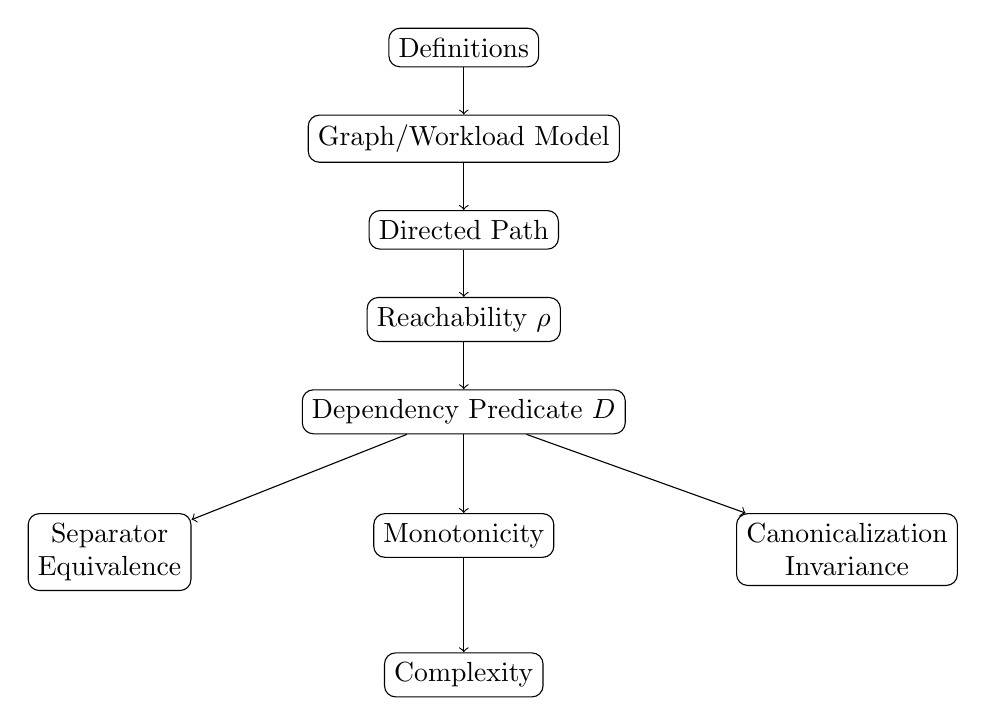
\begin{tikzpicture}[node distance=6mm, every node/.style={draw, rounded corners, align=center, inner sep=3.5pt}]
  \node (defs) {Definitions};
  \node (graph) [below=of defs] {Graph/Workload Model};
  \node (path) [below=of graph] {Directed Path};
  \node (reach) [below=of path] {Reachability $\rho$};
  \node (dep) [below=of reach] {Dependency Predicate $D$};

  \node (sep) [below left=10mm and 14mm of dep] {Separator\\Equivalence};
  \node (mono) [below=10mm of dep] {Monotonicity};
  \node (canon) [below right=10mm and 14mm of dep] {Canonicalization\\Invariance};

  \node (cx) [below=12mm of mono] {Complexity};

  \draw[->] (defs) -- (graph);
  \draw[->] (graph) -- (path);
  \draw[->] (path) -- (reach);
  \draw[->] (reach) -- (dep);
  \draw[->] (dep) -- (sep);
  \draw[->] (dep) -- (mono);
  \draw[->] (dep) -- (canon);
  \draw[->] (mono) -- (cx);
\end{tikzpicture}
\caption{Logical dependency of definitions and theorems.}
\label{fig:theorem-deps}
\end{figure}

\subsection*{Notation}
\begin{center}
\begin{tabular}{@{}ll@{}}
\toprule
\textbf{Symbol} & \textbf{Meaning} \\
\midrule
$G=(V,E)$ & Directed graph \\
$V$ & Components \\
$E$ & Execution relations \\
$R$ & Root set \\
$t$ & Target node \\
$S$ & Candidate component set \\
$w=(R,t,S)$ & Workload \\
$\pi_S(G)$ & Complement projection \\
$\rho$ & Reachability predicate \\
$D(G,w)$ & Dependency predicate \\
$\kappa$ & Canonicalization map \\
\bottomrule
\end{tabular}
\end{center}

\section{Illustrative Diagrams}

Figure~\ref{fig:original-graph} presents a simple execution graph used as a running example. Figure~\ref{fig:remove-b} shows the counterfactual removal step that witnesses dependency by eliminating all $R\leadsto t$ paths. Figure~\ref{fig:pipeline} summarizes the overall dependency analysis pipeline from question to decision.

\begin{figure}[t]
\centering
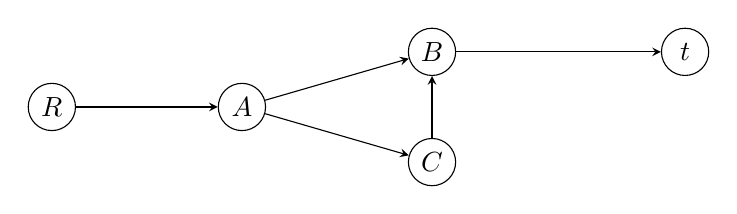
\begin{tikzpicture}[>=stealth, node distance=18mm]
  \tikzstyle{v}=[circle, draw, minimum size=6mm, inner sep=0pt]

  \node[v] (R) {$R$};
  \node[v, right=of R] (A) {$A$};
  \node[v, right=of A, yshift=7mm] (B) {$B$};
  \node[v, right=of A, yshift=-7mm] (C) {$C$};
  \node[v, right=of B, xshift=8mm] (T) {$t$};

  \draw[->] (R) -- (A);
  \draw[->] (A) -- (B);
  \draw[->] (A) -- (C);
  \draw[->] (C) -- (B);
  \draw[->] (B) -- (T);
\end{tikzpicture}
\caption{Original execution graph. Every path from roots $R$ to target $t$ passes through $B$.}
\label{fig:original-graph}
\end{figure}

\begin{figure}[t]
\centering
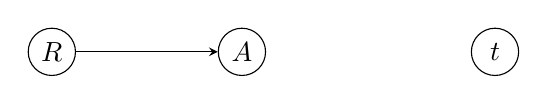
\begin{tikzpicture}[>=stealth, node distance=18mm]
  \tikzstyle{v}=[circle, draw, minimum size=6mm, inner sep=0pt]

  \node[v] (R) {$R$};
  \node[v, right=of R] (A) {$A$};
  \node[v, right=of A, xshift=8mm] (T) {$t$};

  \draw[->] (R) -- (A);
  % No edge into $t$ after removing $B$.
\end{tikzpicture}
\caption{Counterfactual removal of $B$: there is no path from $R$ to $t$, so $D(G,w)=1$.}
\label{fig:remove-b}
\end{figure}

\begin{figure}[t]
\centering
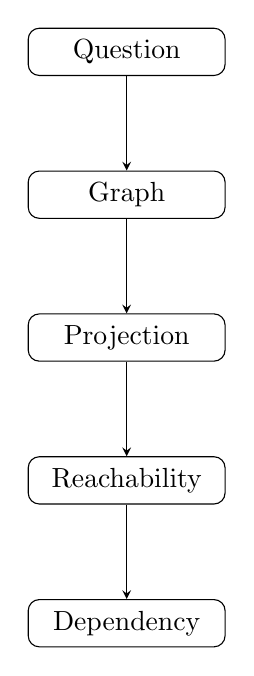
\begin{tikzpicture}[>=stealth, node distance=12mm]
  \tikzstyle{box}=[rectangle, draw, rounded corners, align=center, minimum height=6mm, minimum width=25mm]

  \node[box] (q) {Question};
  \node[box, below=of q] (g) {Graph};
  \node[box, below=of g] (p) {Projection};
  \node[box, below=of p] (r) {Reachability};
  \node[box, below=of r] (d) {Dependency};

  \draw[->] (q) -- (g);
  \draw[->] (g) -- (p);
  \draw[->] (p) -- (r);
  \draw[->] (r) -- (d);
\end{tikzpicture}
\caption{Pipeline view: dependency is decided by graph construction, projection, and reachability.}
\label{fig:pipeline}
\end{figure}

\section{Definitions}
\label{sec:definitions}
Let \(W\) denote a workload and let \(S\) denote a candidate component or component set.

\begin{definition}[Dependency (informal)]
A workload \(W\) forms a dependency on \(S\) when removing \(S\) eliminates all root-to-target directed paths relevant to \(W\).
Section~\ref{sec:dependency-predicate} makes this precise via the projection operator $\pi_S$ and the reachability predicate $\rho$.
\end{definition}

\begin{definition}[Removal-Sensitive Execution Integrity]
Dependency is not an intrinsic property of a component.
It is a property of execution topology under removal perturbation.
\end{definition}
\section{Canonical Graph Model}
\label{sec:graph-model}
We separate (i) the graph model, (ii) the workload model, and (iii) the canonical structural object.

\subsection{Graph}
We model a system as a finite directed graph
\[
G=(V,E),
\]
where \(V\) is a finite set of components and \(E\subseteq V\times V\) is a set of directed relations.

\begin{definition}[Directed path]
\label{def:directed-path}
A (finite) directed path from \(u\in V\) to \(v\in V\) is a finite sequence
\(P=(v_0,\dots,v_k)\) with \(v_0=u\), \(v_k=v\), and \((v_i,v_{i+1})\in E\) for all \(0\le i<k\).
\end{definition}

\subsection{Workload}
A workload is represented as
\[
w=(R,t,S),
\]
where \(R\subseteq V\) is a set of its roots, \(t\in V\) is a target, and \(S\subseteq V\) is the candidate component set being tested.

\subsection{Canonical structural object}
The canonical structural object is
\[
\Sigma=(G,\mathcal{W},\kappa),
\]
where \(\mathcal{W}\) is a set of workloads and \(\kappa\) is a canonicalization map that normalizes equivalent concrete descriptions into deterministic structural representations.
\section{Dependency Predicate}
\label{sec:dependency-predicate}
The dependency predicate is defined through counterfactual removal.

Let
\[
\pi_S(G)
\]
denote the graph obtained by removing every component in the candidate
set \(S\) together with all incident execution edges.

Define the reachability predicate
\[
\rho(G,R,t)=1
\iff
\exists r\in R\;\exists P:r\leadsto t\text{ in }G,
\]
and otherwise \(\rho(G,R,t)=0\), where \(P:r\leadsto t\) denotes a finite directed path (Definition~\ref{def:directed-path}).

\begin{definition}[Dependency Predicate]

A candidate component set \(S\) is a dependency for workload
\(w=(R,t,S)\) if and only if

\begin{equation}
\label{eq:dependency}
D(G,w)=1
\iff
\rho(\pi_S(G),R,t)=0.
\end{equation}

Equivalently, dependency exists precisely when removing \(S\)
eliminates every valid execution path from the workload roots to the
target.

\end{definition}
\subsection{Standing Assumptions}
Unless stated otherwise, throughout the remainder of this paper we assume:
\begin{enumerate}[label=(A\arabic*),leftmargin=*]
  \item $G=(V,E)$ is a finite directed graph.
  \item $\pi_S(G)$ deletes all vertices in $S\subseteq V$ together with their incident edges.
  \item Workloads are terminal-normalized triples $w=(R,t,S)$ with $R\subseteq V$ and $t\in V$.
  \item $\rho(G,R,t)$ denotes directed reachability from some $r\in R$ to $t$.
  \item Canonicalization $\kappa$ is deterministic and dependency queries are evaluated on canonical normal forms.
  \item The execution topology modeled by $G$ is static for the duration of a query.
\end{enumerate}

\section{Separator Equivalence Theorem}
\label{sec:separator}
\begin{theorem}[Dependency--Separator Equivalence]
\label{thm:separator}

Let

\[
G=(V,E)
\]

be a finite directed graph, and let

\[
w=(R,t,S)
\]

be a workload.

Then

\[
D(G,w)=1
\]

if and only if removing every vertex in \(S\) disconnects every path
from the root set \(R\) to the target \(t\).

Equivalently,

\[
D(G,w)=1
\iff
S
\text{ is an }(R,t)\text{-separator}.
\]

\end{theorem}

\begin{proof}
We prove both directions.

($\Rightarrow$) Assume $D(G,w)=1$. By Equation~\ref{eq:dependency},
\(\rho(\pi_S(G),R,t)=0\). Suppose for contradiction that $S$ is \emph{not}
an $(R,t)$-separator in $G$. Then there exists a directed path
$P:r\leadsto t$ in $G$ with $r\in R$ such that $P$ avoids every vertex in
$S$. Deleting $S$ therefore leaves $P$ intact as a directed path in
$\pi_S(G)$, implying $\rho(\pi_S(G),R,t)=1$, a contradiction. Hence $S$
separates $R$ from $t$.

($\Leftarrow$) Assume $S$ is an $(R,t)$-separator in $G$, i.e., every
directed path from any $r\in R$ to $t$ intersects $S$. Then after deleting
$S$, no directed path from $R$ to $t$ can remain in $\pi_S(G)$, so
$\rho(\pi_S(G),R,t)=0$. By Equation~\ref{eq:dependency}, $D(G,w)=1$.
\end{proof}
\section{Monotonicity Theorem}
\label{sec:monotonicity}
\begin{theorem}[Monotonicity of Dependency under Candidate Set Inclusion]
\label{thm:monotonicity}

Let

\[
S \subseteq S'
\]

be candidate component sets for the same workload

\[
w=(R,t,S).
\]

If

\[
D(G,w;S)=1,
\]

then

\[
D(G,w;S')=1.
\]

In other words, once a component set eliminates all directed paths from
the roots to the target, removing additional vertices cannot create a new
root-to-target directed path.

\end{theorem}

\begin{proof}

Fix the same underlying directed graph $G$ and the same roots $R$ and
target $t$ throughout; only the candidate deletion set varies. Assume

\[
S \subseteq S'.
\]

The projection

\[
\pi_{S'}(G)
\]

removes every vertex removed by

\[
\pi_S(G)
\]

and possibly more.

Removing additional vertices cannot create new directed paths between
the workload roots and target.

Therefore,

\[
\rho(\pi_{S'}(G),R,t)
\le
\rho(\pi_S(G),R,t),
\]

where the reachability predicate is interpreted in Boolean order.

If

\[
D(G,w;S)=1,
\]

then

\[
\rho(\pi_S(G),R,t)=0.
\]

Consequently,

\[
\rho(\pi_{S'}(G),R,t)=0,
\]

which implies

\[
D(G,w;S')=1.
\]

Hence dependency is monotone under component deletion.

\end{proof}
\section{Canonicalization Congruence}
\label{sec:canonicalization}
\begin{definition}[Canonicalization]

Let

\[
\kappa : \mathcal{X} \rightarrow \mathcal{N}
\]

be a canonicalization map from concrete structural descriptions
to deterministic normal forms.

Two concrete descriptions

\[
x,y \in \mathcal{X}
\]

are canonically equivalent if

\[
\kappa(x)=\kappa(y).
\]

\end{definition}
\begin{proposition}[Canonicalization assumptions]
\label{prop:canonicalization-assumptions}
Throughout this section we assume:
\begin{enumerate}[label=(C\arabic*),leftmargin=*]
  \item \textbf{Semantic preservation:} normalization preserves graph semantics relevant to $\pi_S$ and $\rho$.
  \item \textbf{Determinism:} $\kappa$ is a deterministic map into a unique normal form.
  \item \textbf{Normalized evaluation:} dependency operators ($\pi_S$, $\rho$, and hence $D$) are evaluated only on normalized graphs.
\end{enumerate}
\end{proposition}

\begin{theorem}[Invariance of Dependency under Canonicalization]
\label{thm:canonicalization}

If

\[
\kappa(x)=\kappa(y),
\]

then every dependency query produces identical results on both
representations.

Equivalently,

\[
D(\kappa(x),w)
=
D(\kappa(y),w).
\]

\end{theorem}

\begin{proof}
Under Proposition~\ref{prop:canonicalization-assumptions}, dependency queries are evaluated only on the canonical normal
form produced by $\kappa$, i.e., the operators used in the query
($\pi_S$, $\rho$, and hence $D$) are functions of the normalized structure.

Since

\[
\kappa(x)=\kappa(y),
\]

both descriptions normalize to the same canonical graph.

Therefore every projection,

\[
\pi_S(G),
\]

is identical under either representation.

Reachability is therefore identical,

\[
\rho(\pi_S(G),R,t),
\]

and consequently

\[
D(\kappa(x),w)
=
D(\kappa(y),w).
\]

Thus dependency analysis depends only on canonical structural
identity rather than incidental serialization.

\end{proof}
\section{Complexity Analysis}
% (duplicate section heading removed)

The dependency predicate admits straightforward complexity bounds.

A single dependency query consists of computing a complement projection
followed by a reachability search.

Using an adjacency-list representation together with either depth-first
or breadth-first search, evaluation requires

\[
O(|V|+|E|)
\]

time and

\[
O(|V|)
\]

space.

Verifying a proposed dependency set therefore has linear complexity.

The computational complexity therefore depends primarily on the chosen analysis task rather than on the dependency predicate itself.

Finding a minimum dependency set reduces to the classical minimum
vertex-cut problem under Theorem~\ref{thm:separator} and is therefore
solvable using established polynomial-time graph algorithms.


Enumerating every dependency set is exponential in the worst case,
since the search space is the power set

\[
2^{|V|}.
\]

Consequently, the contribution of this work is not a new complexity
class but a deterministic structural formulation of dependency over
canonical graph representations.
\section{Relationship to Prior Work}
% (duplicate section heading removed)

The dependency predicate developed in this paper is grounded in
established graph theory.

The separator equivalence theorem follows directly from classical
results relating vertex separators and reachability (e.g., via Menger-style
connectivity arguments) \cite{menger1927}.

Likewise, the single-entry special case closely resembles dominator
theory in compiler construction, where every execution path must pass
through a distinguished vertex \cite{lengauer1979}.

Program Dependence Graphs (PDGs) and Code Property Graphs (CPGs)
demonstrate that structural graph representations are effective
substrates for static program analysis \cite{ferrante1987,yamaguchi2014cpg}.

We compare these settings because they exemplify three complementary roles for ``dependency'' graphs: PDGs/CPGs as analysis-oriented program structure, LLVM as a widely used concrete substrate on which such analyses are executed, and PROV as an interoperability-oriented vocabulary for causal and provenance assertions. The present work abstracts these traditions to a minimal reachability-and-separation interface, making explicit which claims depend on the workload definition versus on the underlying graph representation.

At the implementation level, concrete compiler IRs such as LLVM provide
standardized graph-like execution structure on which these analyses can be
realized \cite{llvmLangRef}.

More broadly, provenance frameworks such as W3C PROV provide graph-based
vocabularies for describing causal structure and dependency-like relations
in heterogeneous systems \cite{w3cprov}.

The contribution of this paper is therefore not a new graph-theoretic
primitive. Rather, it combines workload-aware dependency analysis,
canonical structural representations, and deterministic normalization
into a unified mathematical framework suitable for structural analysis.
\section{Discussion}
% (duplicate section heading removed)

The mathematical results presented here deliberately make conservative
claims.

The dependency predicate is expressed entirely in terms of graph
projection and reachability and therefore inherits the strengths and
limitations of graph-theoretic reasoning.

\paragraph{Limitations.}
The model abstracts away dynamic behavior (e.g., time, probabilistic
failure, retries, and adaptation) and treats execution structure as a
static directed graph. The workload interface $w=(R,t,S)$ captures only
root-to-target reachability and does not encode quantitative notions of
partial service, alternative targets, or degrees of degradation. In
addition, canonicalization is treated axiomatically via $\kappa$ rather
than constructed for a specific concrete system representation.

\subsection*{Future Work}
Several extensions appear natural:
\begin{itemize}[leftmargin=*,nosep]
  \item \textbf{Degradation gradient:} replace the Boolean reachability predicate
  with a graded notion of service loss (e.g., path counts, costs, or
  probabilistic connectivity) to measure partial dependency.
  \item \textbf{Set-valued dependency:} allow multiple targets or target sets and
  characterize dependencies that preserve some subset of objectives.
  \item \textbf{Substitution operators:} model replacement and redundancy by adding
  operators that modify $G$ (or $\pi_S$) while preserving canonicalization.
  \item \textbf{Benchmark validation:} instantiate $\kappa$ and $G$ for real systems
  (e.g., compiler IR graphs, supply-chain graphs) and evaluate how well the
  predicate predicts observed breakage under removal.
\end{itemize}
\section{Conclusion}
% (duplicate section heading removed)

This paper formalizes dependency as a workload-relative
deletion/reachability predicate over canonical structural graphs.

The resulting theory establishes formal definitions, separator
equivalence, monotonicity, canonicalization congruence, and complexity
bounds while remaining consistent with established graph theory.

The work does not claim a new computational primitive.

Instead, it provides a rigorous mathematical foundation for
deterministic structural dependency analysis and establishes a basis
upon which richer structural-analysis and execution-governance systems
may be developed.

This work establishes a mathematical foundation for dependency as a workload-relative graph property. Future work may extend the model to graded dependency, substitution algebras, dynamic systems, and richer structural analyses while preserving the deterministic framework introduced here.

\appendix

\refstepcounter{section}
\section*{Appendix \thesection\\Worked Example}
\label{app:worked-example}
Consider a directed graph $G=(V,E)$ with $V=\{r,a,b,t\}$ and
$E=\{(r,a),(a,t),(r,b),(b,t)\}$. Let the workload be $w=(R,t,S)$ with
$R=\{r\}$ and candidate set $S=\{a\}$.

The projection $\pi_S(G)$ deletes $a$ and all incident edges, yielding the remaining edges $\{(r,b),(b,t)\}$. Since a directed path $r\leadsto t$ (namely $r\to b\to t$) still exists in $\pi_S(G)$, we have $\rho(\pi_S(G),R,t)=1$ and therefore $D(G,w)=0$.

If instead $S'=\{a,b\}$, then $\pi_{S'}(G)$ deletes both internal vertices and no directed path from $r$ to $t$ remains. Hence $\rho(\pi_{S'}(G),R,t)=0$ and $D(G,(R,t,S'))=1$.

\refstepcounter{section}
\section*{Appendix \thesection\\Notation Index}
\label{app:notation}
\begin{center}
\begin{tabular}{@{}ll@{}}
\toprule
\textbf{Symbol} & \textbf{Meaning} \\
\midrule
$G=(V,E)$ & Directed graph \\
$V$ & Components \\
$E$ & Execution relations \\
$R$ & Root set \\
$t$ & Target node \\
$S$ & Candidate component set \\
$w=(R,t,S)$ & Workload \\
$\pi_S(G)$ & Complement projection \\
$\rho(G,R,t)$ & Reachability predicate \\
$D(G,w)$ & Dependency predicate \\
$\kappa$ & Canonicalization map \\
$\Sigma$ & Canonical structural object $(G,\mathcal{W},\kappa)$ \\
$\mathcal{W}$ & Workload set \\
\bottomrule
\end{tabular}
\end{center}

\bibliographystyle{plain}
\bibliography{references}

\end{document}
